\subsection{Sequence diagrams}
\subsubsection{Xác thực}
\begin{figure}[H]
    \begin{center}
        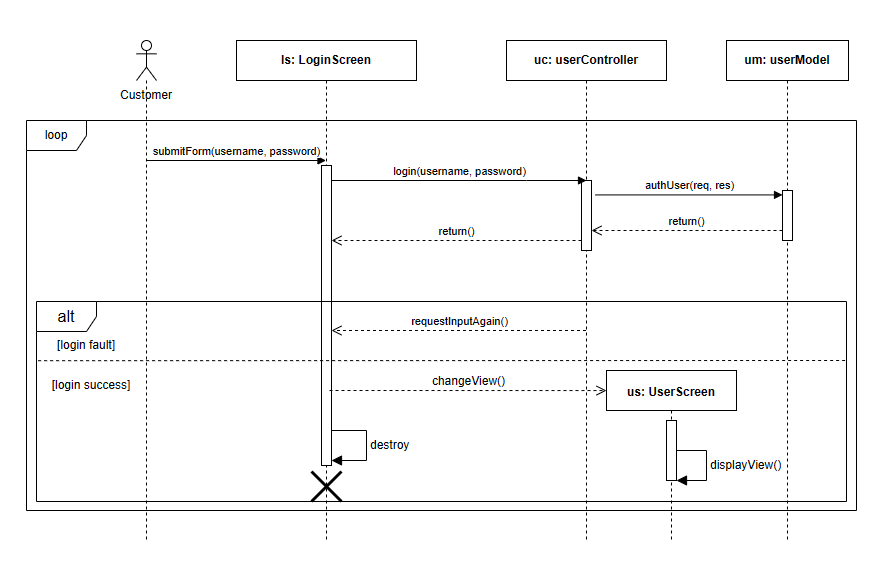
\includegraphics[width=0.9\textwidth]{Images/System Modelling/Authen_Sequence.png}
        \caption{Sequence diagram cho module xác thực tài khoản}
    \end{center}
\end{figure}
\textbf{Mô tả: }\par
Đầu tiên, Customer sẽ nhập username vs password thông qua hàm submitForm(username, password). uc sẽ gọi hàm login(username, password) để tiếp nhận giá trị của username và password. uc sẽ yêu cầu um gọi hàm authUser(req, res) để xác thực username và password và trả giá trị về ls.
Nếu giá trị sai sẽ yêu cầu nhập lại username và password, nếu giá trị đúng sẽ trả về giao diện của user.


\subsubsection{In}
\begin{figure}[H]
    \begin{center}
        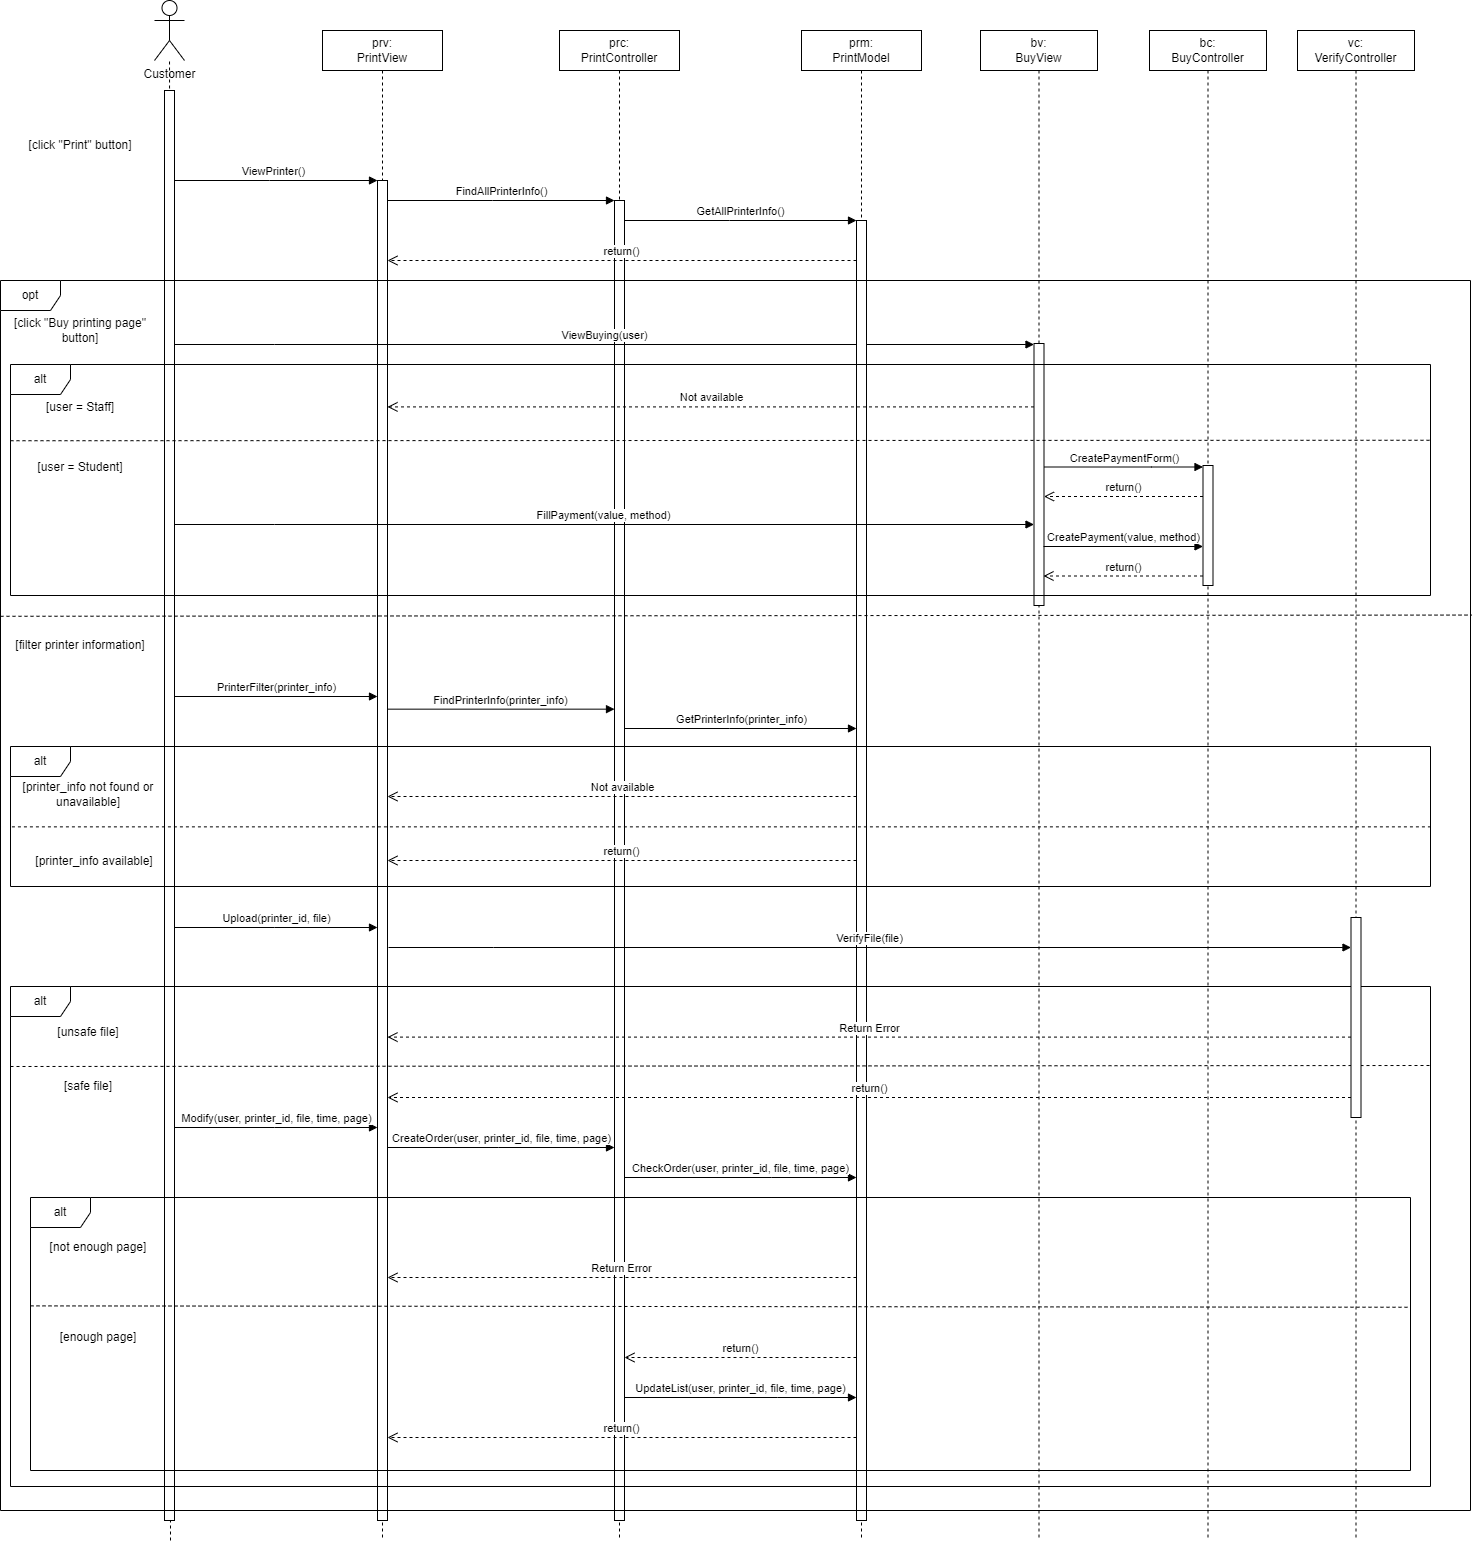
\includegraphics[width=1\textwidth]{Images/System Modelling/Printing_Sequence.png}
        \caption{Sequence diagram cho module in}
    \end{center}
\end{figure}
\textbf{Mô tả: }\par
Đầu tiên, Customer sẽ mở \textbf{prv} qua hàm \textit{ViewPrinter()}. Sau đó \textbf{prc} gọi hàm \textit{FindAllPrinterInfo()} để lấy tất cả máy in hiển thị trên \textbf{prv}. \\
\textbf{prc} yêu cầu \textbf{prm} gọi hàm \textit{GetAllPrinterInfo()} để lấy danh sách máy in từ database, sau đó danh sách máy in sẽ được trả về và hiển thị ở \textbf{prv}.
Tiếp theo Customer có 2 luồng lựa chọn song song:
\begin{enumerate} [1. ]
    \item Customer click vào "Mua thêm giấy", mở \textbf{bv} qua hàm \textit{ViewBuying(user)}. 
    \begin{itemize}
        \item Nếu như user truyền vào là Staff thì sẽ báo lỗi về \textbf{prv} và hiển thị lên màn hình.
        \item Nếu user truyền vào là Student, \textbf{bv} yêu cầu \textbf{bc} gọi hàm \textit{CreatePaymentForm()} để tạo form thông tin thanh toán, sau đó trả về màn hình. Tiếp theo Customer cung cấp thông tin thanh toán bao gồm số lượng giấy và phương thức thanh toán và gọi hàm \textit{FillPayment(value, method)} từ \textbf{bv}, sau đó \textbf{bv} yêu cầu \textbf{bc} gọi hàm \textit{CreatePayment(value, method)}, xử lý với hệ thống thanh toán và trả về màn hình kết quả giao dịch.
    \end{itemize}

     \item Customer tiến hành lọc thông tin của máy in, \textbf{prv} sẽ gọi hàm \textit{PrinterFilter(printer\_info)} dựa trên thông tin vừa được lọc, sau đó \textbf{prc} gọi hàm \textit{FindPrinterInfo(printer\_info)} để tìm những máy in phù hợp hiển thị lên màn hình. Tiếp theo \textbf{prc} yêu cầu \textbf{prm} gọi hàm \textit{GetPrinterInfo(printer\_info)} để lấy danh sách máy in trong database phù hợp với thông tin được cung cấp.
     \begin{itemize}
         \item Nếu không tìm được máy in phù hợp với thông tin lọc hoặc nếu có mà (các) máy in đó đang được bảo trì thì sẽ báo lỗi về \textbf{prv} và hiển thị lên màn hình.
         \item Ngược lại, trả kết quả về \textbf{prv} và hiển thị danh sách các máy in phù hợp lên màn hình.
     \end{itemize}
     Customer chọn vào máy muốn in và upload tài liệu. Sau đó \textbf{prv} sẽ gọi hàm \textit{Upload(printer\_id, file)} và yêu cầu \textbf{vc} gọi hàm \textit{VerifyFile(file)} để xác minh nội dung của file vừa được upload.
     \begin{itemize}
         \item Nếu file vừa up có nội dung không an toàn, \textbf{vc} sẽ báo lỗi về \textbf{prv} và hiển thị lên màn hình.
         \item Ngược lại, \textbf{vc} trả kết quả xác minh thành công và hiển thị lên màn hình. Sau đó Customer sẽ định dạng và cung cấp các thông tin in (thời gian, số lượng trang cần in), \textbf{prv} sẽ gọi hàm \textit{Modify(user, printer\_id, file, time, page)}, sau đó \textbf{prc} sẽ tạo order bằng hàm \textit{CreateOrder(user, printer\_id, file, time, page)} và yêu cầu \textbf{prm} gọi hàm \textit{CheckOrder(user, printer\_id, file, time, page)} để truy xuất vào database kiểm tra thông tin in của Customer.
         \begin{itemize}
             \item Nếu số lượng giấy của Customer không đủ, \textbf{prm} sẽ báo lỗi về \textbf{prv} và hiển thị lên màn hình.
             \item Ngược lại, \textbf{prm} trả kết quả về \textbf{prc}, sau đó \textbf{prc} sẽ tiếp tục yêu cầu \textbf{prm} gọi hàm \textit{UpdateList(user, printer\_id, file, time, page)} để cập nhật thông tin in vào database. Cuối cùng \textbf{prm} trả kết quả về \textbf{prv} và hiển thị lên màn hình.
         \end{itemize}
     \end{itemize}
\end{enumerate}

\subsubsection{Quản lý máy in}
\begin{figure}[H]
    \begin{center}
        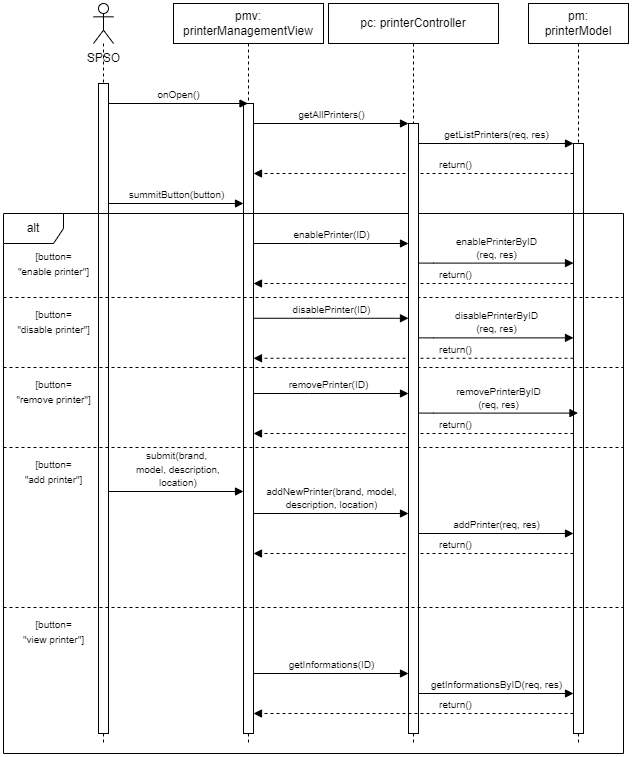
\includegraphics[width=0.9\textwidth]{Images/System Modelling/PM_Sequence.png}
        \caption{Sequence diagram cho module quản lý máy in}
        \label{fig:arch}
    \end{center}
\end{figure}
\textbf{Mô tả:}\par
1. Đầu tiên, pmv sẽ được mở bởi SPSO qua hàm onOpen().\par
2. pc gọi hàm getAllPrinters() để lấy tất cả máy in để hiển thị trên pmv. \par
3. pc yêu cầu pm gọi hàm getListPrinters() để lấy danh sách các máy in từ database. \par
4. Danh sách các máy in sẽ được return() và hiển thị ở pmv. \par
\textbf{Tại bước 5: có 5 lựa chọn}\par
\textbf{A1:}\par
5. SPSO chọn nút "enable printer" nên pmv gọi hàm submit("enable printer").\par
6. pc gọi hàm enablePrinter(ID) ứng với ID của máy in được chọn để kích hoạt máy in.\par
7. pm gọi hàm enablePrinterByID(req, res) từ yêu cầu của pc để set giá trị state của máy in thành 1.\par
8. Dữ liệu được cập nhật, return() và hiển thị ở pmv.\par
\textbf{A2:}\par
5. SPSO chọn nút "disable printer" nên pmv gọi hàm submit("disable printer").\par
6. pc gọi hàm disablePrinter(ID) ứng với ID của máy in được chọn để vô hiệu hóa máy in.\par
7. pm gọi hàm disablePrinterByID(req, res) từ yêu cầu của pc để set giá trị state của máy in thành 0.\par
8. Dữ liệu được cập nhật, return() và hiển thị ở pmv.\par
\textbf{A3:}\par
5. SPSO chọn nút "remove printer" nên pmv gọi hàm submit("remove printer").\par
6. pc gọi hàm removePrinter(ID) ứng với ID của máy in được chọn để xóa máy in.\par
7. pm gọi hàm removePrinterByID(req, res) từ yêu cầu của pmc để xóa máy in trong database.\par
8. Dữ liệu được cập nhật, return() và hiển thị ở pmv.\par
\textbf{A4:}\par
5. SPSO chọn nút "add printer" nên pmv gọi hàm submit("add printer").\par
6. SPSO nhập các thông tin của máy in và pmv gọi hàm submit(brand, model, description, location).\par
7. pc gọi hàm addNewPrinter(brand, model, description, location) để thêm máy in mới với các thuộc tính được SPSO nhập.\par
8. pm gọi hàm addPrinter(req, res) từ yêu cầu của pmc để thêm máy in trong database.\par
9. Dữ liệu được cập nhật, return() và hiển thị ở pmv.\par
\textbf{A5:}\par
5. SPSO chọn nút "view printer" nên pmv gọi hàm submit("remove printer").\par
6. pc gọi hàm getInformations(ID) ứng với ID của máy in được chọn để lấy tất cả thông tin của máy in.\par
7. pm gọi hàm getInformationsByID(req, res) từ yêu cầu của pmc để lấy tất cả thông tin của máy in từ database.\par
8. Dữ liệu được lấy, return() và hiển thị ở pmv.\par

\subsubsection{Sửa danh mục định dạng tệp cho phép in}

\begin{figure}[H]
    \begin{center}
        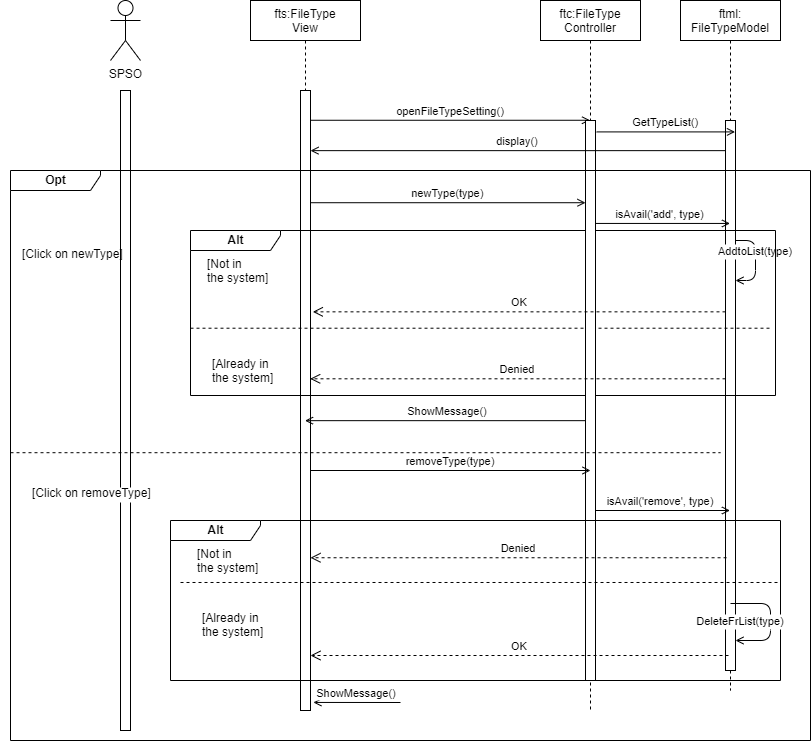
\includegraphics[width=0.9\textwidth]{Images/System Modelling/FileTypeSetting_Sequence.png}
        \caption{Sequence diagram cho module Sửa định dạng tệp cho phép in}
        \label{fig:arch}
    \end{center}
\end{figure}
\textbf{Mô tả:}\par
Khởi đầu flow, SPSO mở FileTypeSetting ở thanh công cụ, hiện thị trong mục Printing management. Hệ thống khởi động màn hình FileTypeView(viết tắt: fts). fts gọi tới bộ phận FileTypeController(viết tắt: fsc) được kích hoạt để gọi lệnh GetTypeList() tới FileTypeModel(ftml), từ đó nhận từ cơ sở dữ liệu danh sách các kiểu file trả về fts và hiển thị cho fts.\par
Tiếp theo, SPSO có 2 luồng lựa chọn song song:
\begin{itemize}
    \item SPSO chọn thêm kiểu file mới với newType(type) trên màn hình fts. ftc sau đó chạy lệnh is\_Avail('add',type) gửi tới ftm, nhằm kiểm tra hệ thống đã có sẵn hoặc chưa có kiểu file mới, nếu ftm xác nhận chưa có kiểu file đó, thực hiện thêm vào cơ sở dữ liệu FileTypeModel(ftml) với AddtoList(), trả về kết quả OK cho ftm và hiển thị thông báo lên màn hình. Ngược lại, nếu kiểu file đã tồn tại trong hệ thống thì trả về denied cho ftm, hiển thị thông báo truy vấn bị từ chối.
    \item SPSO chọn xóa kiểu file đang có với removeType(type) trên màn hình. ftm sau đó chạy lệnh delete(type) gửi tới ftm, nhằm kiểm tra hệ thống đã có sẵn hoặc chưa có kiểu file mới, ftm gọi ftc kiểm tra với truy vấn isAvail(type), nếu hệ thống đã có kiểu file đó, thực hiện xóa khỏi cơ sở dữ liệu ftml với DeletefrList(type), trả về kết quả OK cho ftm và hiển thị thông báo lên màn hình. Ngược lại, nếu kiểu file chưa tồn tại trong hệ thống thì trả về denied cho ftm, hiển thị thông báo truy vấn bị từ chối.
\end{itemize}
\subsubsection{Quản lý tặng giấy miễn phí}

\begin{figure}[H]
    \begin{center}
        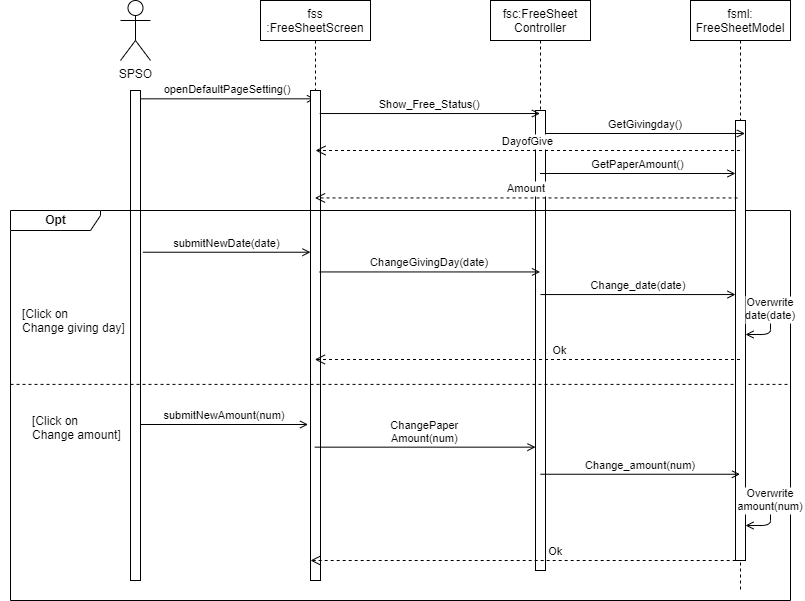
\includegraphics[width=0.9\textwidth]{Images/System Modelling/FreeSheetSetting_Sequence.png}
        \caption{Sequence diagram cho module Quản lý tặng giấy miễn phí}
        \label{fig:arch}
    \end{center}
\end{figure}
\textbf{Mô tả:}\par
Để khởi đầu flow, SPSO mở DefaultPageSetting ở thanh công cụ, xuất hiện trong mục Printing management. Hệ thống khởi động màn hình FreeSheetScreen(viết tắt: fss), từ đây gửi lệnh GetFreeSheetStatus() để lấy thông tin hiện tại về quà tặng giấy miễn phí. Bộ phận FreeSheetManager(viết tắt: fsm) được kích hoạt để gọi 2 lệnh GetGivingDay, GetPaperAmount truy vấn từ FreeSheetController(viết tắt fsc), mục đích là lấy từ cơ sở dữ liệu DayofGive, Amount tương ứng là ngày tặng giấy và số lượng giấy đã được lưu trả về fsm. Sau đó fsm gửi lệnh hiển thị cho fss.  \par
Tiếp theo, SPSO có 2 luồng lựa chọn song song:
\begin{itemize}
    \item Luồng submitNewDate(date) trên fss để thay đổi ngày tháng tặng giấy miễn phí, tham số date là ngày mới được chọn, lệnh được chuyển tiếp tới fsm với ChangeGivingDay(date), chuyển tiếp tới Change\_date cho fsc. Khi fsc đã nhận được lệnh, thực hiện lệnh Overwritedate(date) để thay đổi cơ sở dữ liệu FreeSheetModel. Để kết thúc, fsc gửi tín hiệu OK cho fsm và hiển thị thông tin xác nhận lên fss.
    \item Luồng submitNewAmount(num) trên fss để thay đổi số lượng giấy miễn phí, tham số num là số lượng giấy mới, lệnh được chuyển tiếp tới fsm với ChangePaperAmount(num), chuyển tiếp tới Change\_amount cho fsc. Khi fsc đã nhận được lệnh, thực hiện lệnh Overwriteamount(num) để thay đổi cơ sở dữ liệu FreeSheetModel. Để kết thúc, fsc gửi tín hiệu OK cho fsm và hiển thị thông tin xác nhận lên fss.
\end{itemize}

\subsubsection{Lịch sử in}
\textbf{Mô tả cho sequence diagram cho use case truy cập lịch sử in của Khách hàng:}\par

Đầu tiên, khách hàng điều hướng tới trang Lịch sử In, giao diện lịch sử in gọi hàm onOpen(). Rồi giao diện Lịch sử In sẽ gọi hàm getHistoryLogs() của logController với tham số là ID khách hàng. logController sẽ truy xuất dữ liệu lịch sử in từ cơ sở dữ liệu. Sau khi thu được dữ liệu lịch sử in, logController sẽ trả về dữ liệu cho giao diện để hiển thị cho khách hàng. \par

Nếu khách hàng sử dụng bộ lọc thời gian, giao diện sẽ truyền thêm tham số timePeriod vào hàm getHistoryLogs(). Trước hết, logController sẽ kiểm tra tính hợp lệ của thời gian người dùng nhập vào, nếu không hợp lệ sẽ báo lỗi. Nếu thời gian hợp lệ, logController sẽ lấy dữ liệu lịch sử in từ cơ sở dữ liệu và lọc lại dữ liệu trong khoảng thời gian khách hàng truyền vào. logController sẽ trả về kết quả cho giao diện hiển thị. \par

Nếu khách hàng sử dụng navbar lọc theo status, logInterface sẽ yêu cầu logController gọi hàm getHistoryLogs(status). Rồi logController sẽ truy cập vào cơ sở dữ liệu để lấy dữ liệu lịch sử in theo status và trả kết quả cho giao diện hiển thị.\par

Nếu khách hàng sử dụng bộ lọc theo máy in, logInterface sẽ yêu cầu danh sách các máy in từ logController. Sau đó, logController sẽ truy xuất danh sách các máy in đang hoạt động từ cơ sở dữ liệu và trả về cho giao diện. Khách hàng sẽ chọn các máy in được hiển thị và giao diện sẽ gọi hàm getHistoryLogs() với ID máy in được chọn. logController truy xuất dữ liệu lịch sử in thỏa các bộ lọc từ cơ sở dữ liệu và trả về cho giao diện hiển thị.\par

\begin{figure}[H]
    \begin{center}
        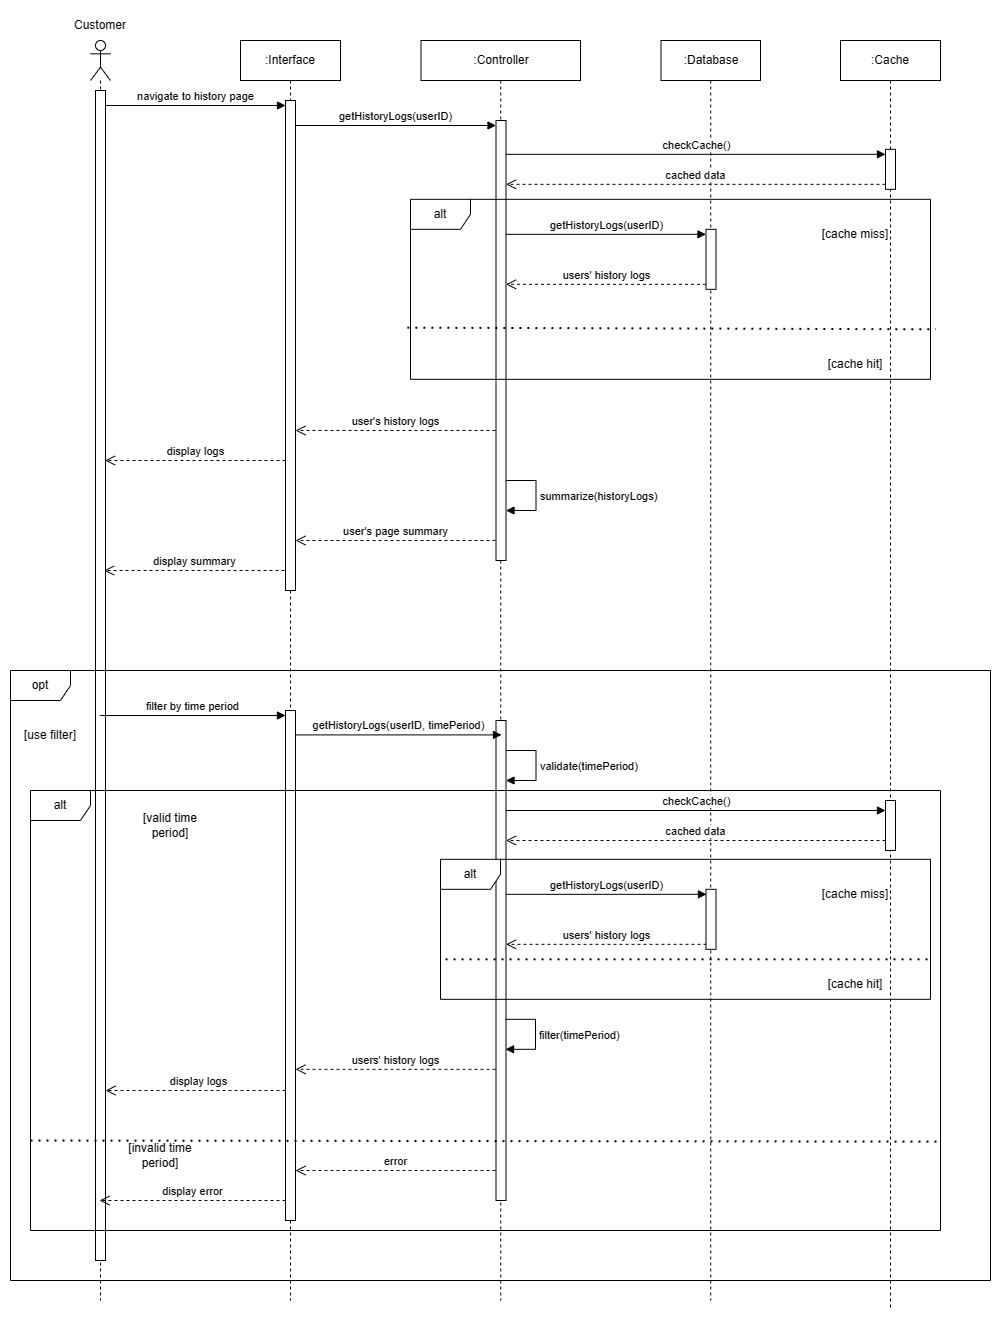
\includegraphics[width=0.77\textwidth]{Images/System Modelling/Logging(customer)_Sequence.png}
        \caption{Sequence diagram cho use case truy cập lịch sử in của Khách hàng}
        \label{fig:arch}
    \end{center}
\end{figure}

\begin{figure}[H]
    \begin{center}
        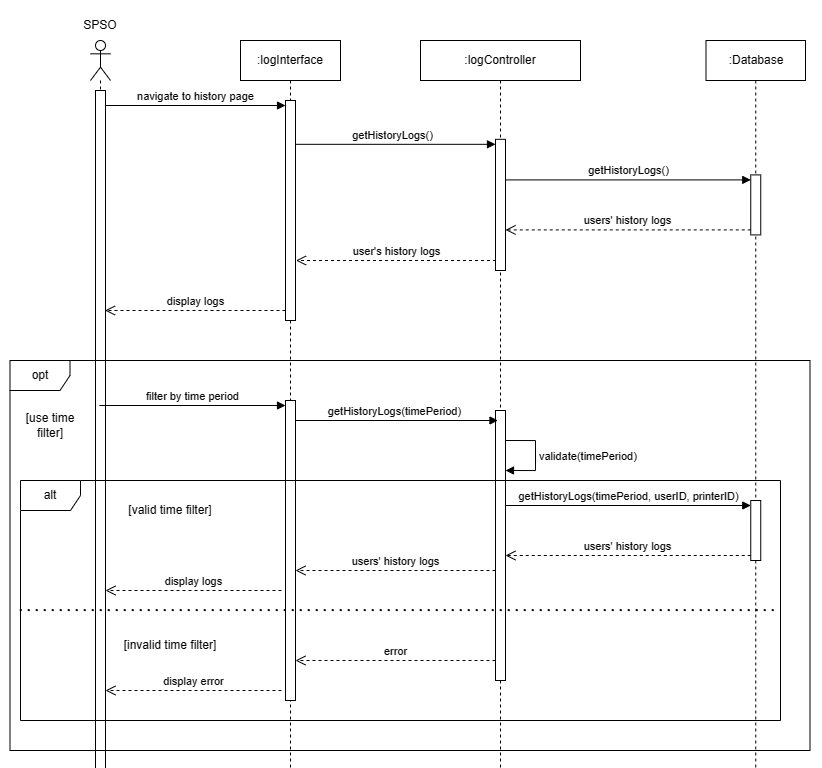
\includegraphics[width=0.7\textwidth]{Images/System Modelling/Logging(SPSO)_Sequence(1).png}
        \caption{Sequence diagram cho use case truy cập lịch sử in của SPSO}
        \label{fig:arch}
    \end{center}
\end{figure}

\textbf{Mô tả:}\par

Đầu tiên, SPSO điều hướng tới trang Lịch sử In, giao diện lịch sử in gọi hàm onOpen(). Rồi giao diện Lịch sử In sẽ gọi hàm getHistoryLogs() của logController. logController sẽ truy xuất dữ liệu lịch sử in từ cơ sở dữ liệu. Sau khi thu được dữ liệu lịch sử in, logController sẽ trả về dữ liệu cho giao diện để hiển thị cho SPSO. \par

Nếu SPSO sử dụng bộ lọc thời gian, giao diện sẽ truyền thêm tham số timePeriod vào hàm getHistoryLogs(). Trước hết, logController sẽ kiểm tra tính hợp lệ của thời gian người dùng nhập vào, nếu không hợp lệ sẽ báo lỗi. Nếu thời gian hợp lệ, logController sẽ lấy dữ liệu lịch sử in từ cơ sở dữ liệu và lọc lại dữ liệu trong khoảng thời gian SPSO truyền vào. logController sẽ trả về kết quả cho giao diện hiển thị. \par

Nếu SPSO sử dụng navbar lọc theo status, logInterface sẽ yêu cầu logController gọi hàm getHistoryLogs(status). Rồi logController sẽ truy cập vào cơ sở dữ liệu để lấy dữ liệu lịch sử in theo status và trả kết quả cho giao diện hiển thị.\par

Nếu SPSO sử dụng bộ lọc theo userID, logInterface sẽ gọi hàm getHistoryLogs() của logController với tham số userID. Trước hết, logController sẽ kiểm tra xem người dùng có tồn tại trong userDatabase hay không. Nếu có, logController sẽ truy xuất dữ liệu từ cơ sở dữ liệu và trả về dữ liệu cho giao diện hiển thị. \par

Nếu SPSO sử dụng bộ lọc theo máy in, logInterface sẽ yêu cầu danh sách các máy in từ logController. Sau đó, logController sẽ truy xuất danh sách các máy in đang hoạt động từ cơ sở dữ liệu và trả về cho giao diện. SPSO sẽ chọn các máy in được hiển thị và giao diện sẽ gọi hàm getHistoryLogs() với ID máy in được chọn. logController truy xuất dữ liệu lịch sử in thỏa các bộ lọc từ cơ sở dữ liệu và trả về cho giao diện hiển thị.\par